\section{Learning How to Refine High-Level Plans}
%% Randomized refinement provides us with a framework to learn a policy
%% that implements \textsc{NDGetInstantiation} and performs well
%% empirically. We apply {\sc rl} to train continuous proposal
%% distributions for symbolic reference instantiations.

\subsection{Formulation as Markov Decision Process}
We formulate plan refinement as the following {\sc mdp}:
\begin{tightlist}
\item States are tuples $\langle \pi, \sigma, E \rangle$ that consist of the
high-level plan, its current (potentially infeasible) refinement, and the
geometric environment.
\item Actions are pairs $\langle p, x \rangle$, where $p$ is the discrete symbolic
reference to resample and $x$ is the continuous value assigned to $p$ in the new refinement.
\item The transition distribution is defined by setting $p$'s value
  to $x$. If $x$ is {\sc ik} feasible, the motion planner determines
  any corresponding trajectories.
\item The reward function $R(s, a, s')$ is linearly interpolated
  between 0 and 20 based on the fraction of high-level actions whose
  preconditions are satisfied. Actions that result in an {\sc ik}
  infeasible pose receive reward $-1$.
\item The horizon is the number of available samples.
\item $\Prob$ is a distribution over plans to be refined, defined as a
  distribution over planning problems.
\end{tightlist}

As an example, consider refining a pick-place high-level plan, where the
robot grasps an object and puts it down at a certain location. The
initial state consists of this plan, a list of initialized parameters,
and meshes that describe the geometry of the problem. We'll suppose
that the initial grasp is infeasible for both the pick and the putdown
actions. The first action selects a new grasp, but receives no reward
because it does not work with the current pick or putdown poses. The
two actions set values for these poses that work with the grasp. The
final step collects the maximum reward of 20 because all instantiated
actions are feasible.

% \begin{figure}[t]
%   \centering
%     \noindent
%     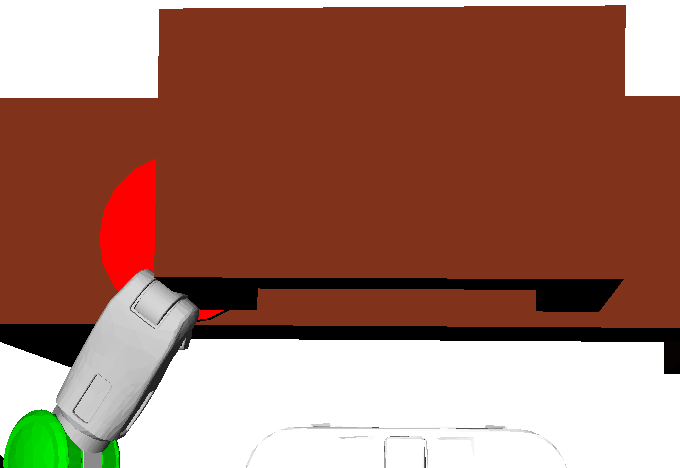
\includegraphics[scale=0.15]{images/fry_bad_grasp_pd1.png}\hspace{6mm}
%     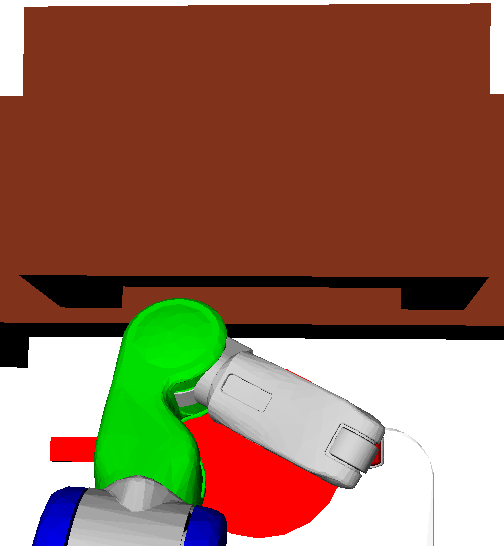
\includegraphics[scale=0.15]{images/fry_bad_grasp_pd2.png}
%     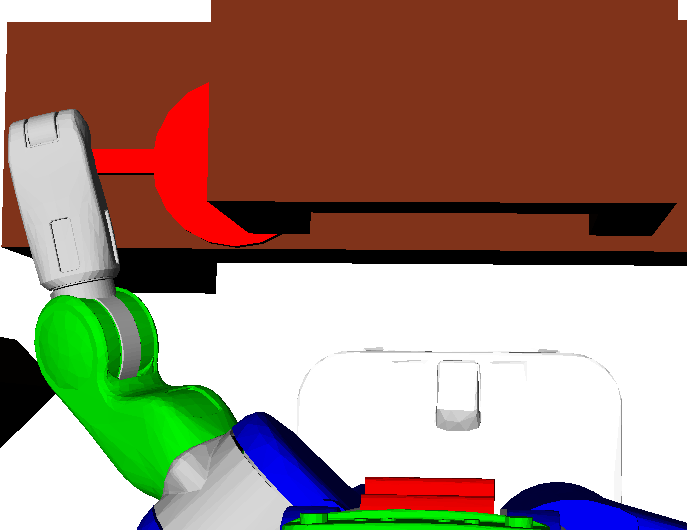
\includegraphics[scale=0.16]{images/fry_good_grasp_bad_pd.png}\hspace{6mm}
%     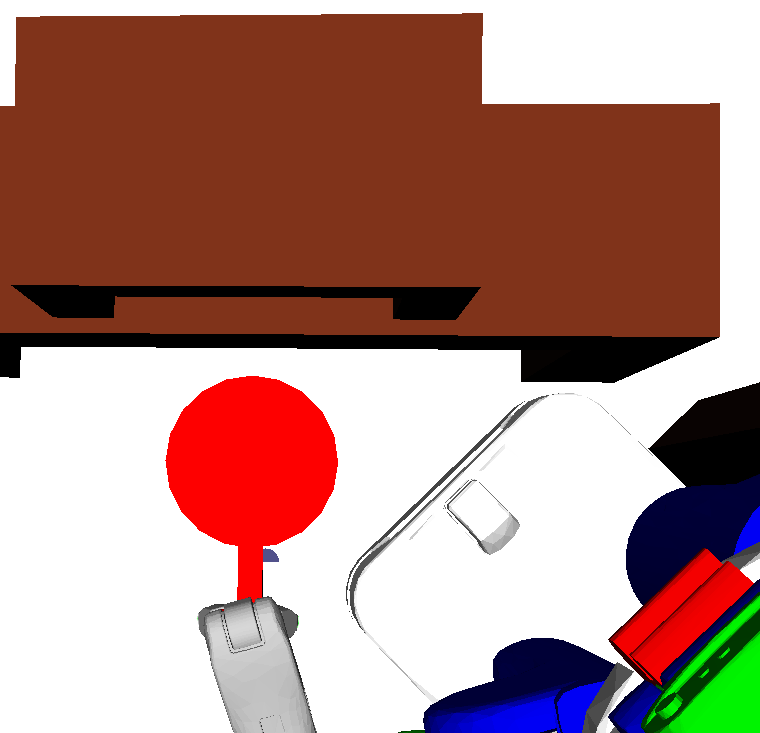
\includegraphics[scale=0.13]{images/fry_good_grasp_good_pd.png}
%   \caption{\small{\textbf{Top}: When the frying pan is not grasped by the handle, any attempted putdown pose for
% placing it into the narrow shelf fails. \textbf{Bottom}: When the frying pan is grasped by the handle, some putdown
% poses may succeed, as in the right, and some may fail, as in the left. In general, delayed rewards
% are important in the plan refinement {\sc mdp}; sometimes multiple symbolic references require resampling to
% change an infeasible refinement into a feasible one.}}
%   \label{fig:delayed}
% \end{figure}

\subsection{Training Process}
We restrict our attention to training policies that suggest $x$ for a
given parameter, since our refinement algorithm defines a way to select
$p$. Our approach is to adapt the method of Zucker et
al.~\cite{workspacebias}, which uses a linear combination of features
to define a distribution over poses. We learn a weight vector
$\theta_{p}$ for each reference \emph{type}, comprised of a pose type
and possibly a gripper (e.g., ``left gripper grasping pose,'' ``right
gripper putdown pose,'' ``base pose'').

We use a feature function $f(s, a) = f(s, p, x)$ that maps the current
state $s \in \St$ and action $a \in \A$ to a feature vector; $f$
defines a policy class for the {\sc mdp}. Additionally, we define $N$
as the number of planning problems on which to train and $\epsilon$ as
the number of samples comprising a training episode, after which we
update weights.

The training is a natural extension of randomized refinement and
progresses as follows. $N$ times, sample from $\Prob$ to obtain a
complete planning problem $\Pi$. For each $\Pi$, compute a high-level plan
and run randomized refinement to attempt to find a valid
plan refinement. Select actions according to the $\theta_{p}$ and
collect rewards according to $R$. After every $\epsilon$ calls to
\textsc{Resample}, take a gradient step on $\theta_{p}$.

For a symbolic reference $p$, in state $s$, our policy selects a
sample value $x$ with probability
$$q(s, p, x) \propto \exp(\theta_{p}^{\top} f(s, p, x)).$$

We define the expected reward of an episode, $\xi$, as
$\eta(\theta_{p})~=~\mathbb{E}_{q}[R(\xi)],$ and approximate its
gradient:
$$\nabla \eta(\theta_{p}) \approx \frac{R(\xi)}{\epsilon}
\sum_{i=1}^{\epsilon}(f(s, p, x_{i}) - \mathbb{E}_{q,s}[f]).$$
$R(\xi)$ is the sum over all rewards obtained throughout $\xi$, and
$\mathbb{E}_{q,s}[f]$ is the expected feature vector under $q$ in
state $s$. Then, for an appropriate step size $\alpha$ the weight
vector update is:
$$\theta_{p} \leftarrow \theta_{p} + \alpha \nabla \eta(\theta_{p}).$$

We sample $x$ from $q$ using the Metropolis algorithm~\cite{chib1995understanding}.
Since our distributions are continuous, calculating $\mathbb{E}_{q,s}[f]$ is hard,
so we approximate it with a Monte Carlo estimate.
